\documentclass[12pt,letterpaper]{article}
\usepackage{fullpage}
\usepackage{lipsum}
\usepackage{graphicx}
\usepackage{float}

\begin{document}
\title{The Eh-P's: Beam Line for Schools Proposal}
\author{
Ryan Marks\\
Jiarui Pu \\ 
Andrew Tan\\
Eric Ye\\
\\
Mentor: Mr. Henri van Bemmel\\
\normalsize{\texttt{hmvb15@rogers.com}}
}

\date{\today}
\maketitle

``Everyone stand back!" we shouted, as we cranked up the voltage knob on the power supply.

It was the third consecutive day we were spending after-school at one of our lab member’s home. We had been working on our physics lab, when we got bored and decided do something else with the coils and power supply.

The lab was on alternating current. We’d read up on topics from capacitors to inductors, transformation of voltage to Maxwell's equations.
And we realized that if we put enough of our coils together in the right way, we could build a transformer that upconverted the voltage hundreds of times. We held two terminals of the wire apart with rubber clamps, and flicked on the switch.

Between the wires, and in our eyes, there were sparks.
\section{Theory}
Our small experiment with alternating current piqued our interest in electromagnetism. Specifically, we were interested in the interpretation of relativistic magnetism our teacher introduced us to. 
This interpreation says that on two parallel current-carrying wires, the negative charges on one wire would 'see' either the positive charge density or negative charge density increase on the other wire depending on the relative motion of the charges due to Lorentz contraction.
Combined with the associated electrostatic forces, this interpretation results in the same outcome as the classical interpretation of electromagnetism.
The experiments we propose will investigate the properties of both these interpretations using of lines of charged particles.

Based on relativistic electromagnetism, we would be expected that the magnetic force from these wires depends on the relative speeds of the charges moving through them.
We propose a series of experiment to determine whether lines of moving charges, such as in beam lines, produce B-fields and if so, whether the B-fields act on other charges moving at the same velocity or stationary objects.

\section{Proposed Experiments}
The goal of these experiments is to investigate the properties of charged particle beams as currents.

\subsection{Experiment 1}
\begin{figure}[H]
\label{experiment_setup1}
  \centering
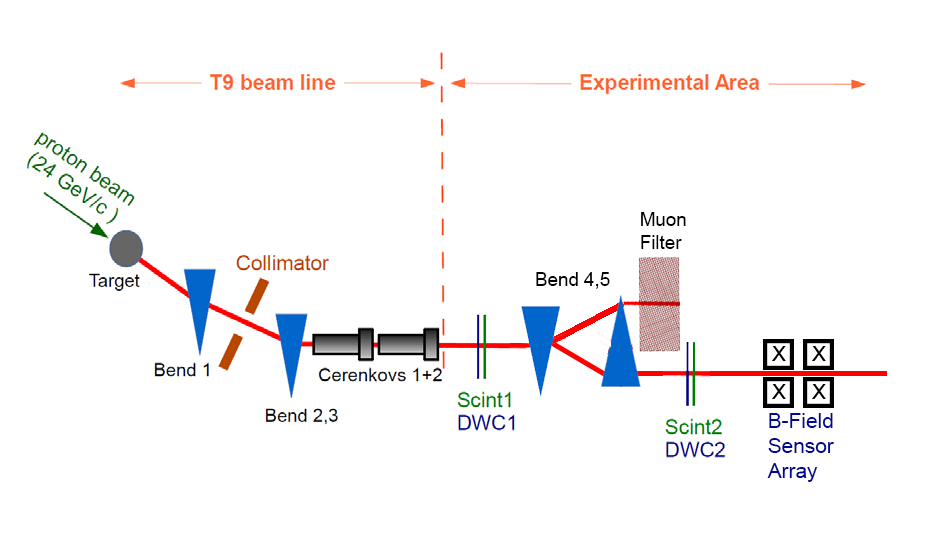
\includegraphics[]{experimental_setup1.png} %is there any reason for the muon filter?
 \caption{The proposed beam line arrangement for experiment 1.}
\end{figure}
First, a line of positive charges will pass by an array of magnetic field sensors in order to determine whether any B field is generated. Since the sensors are stationary while the particles are moving at relativistic speeds, a B-field dependent on the momenta of the particles would be expected.

\subsection{Experiment 2}
\begin{figure}[H]
\label{experiment_setup2}
  \centering
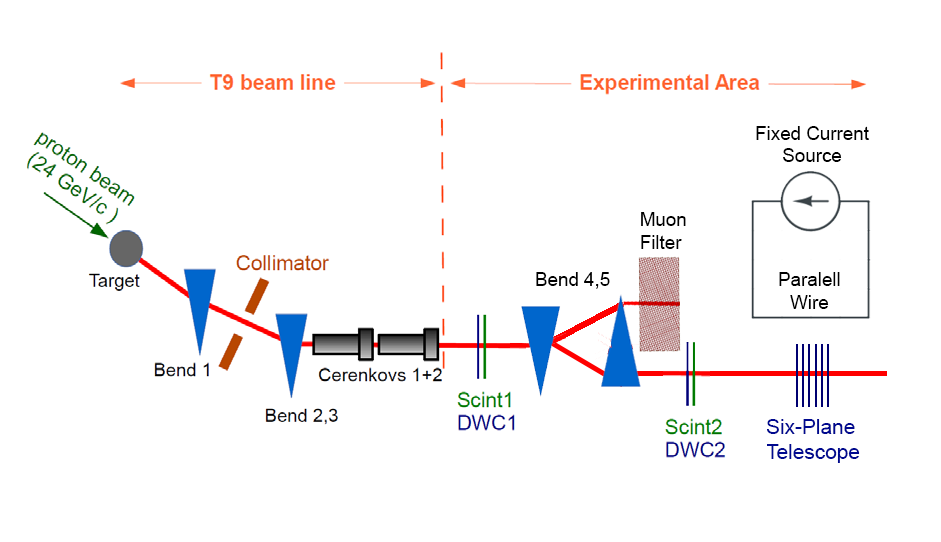
\includegraphics[]{experimental_setup2.png}
 \caption{The proposed beam line arrangement for experiment 2.}
\end{figure}
The second experiment will effectively verify the Hall Effect with particle beams.
%why the hall effect? Aren't we just looking at forces? Shouldn't hall effect be in experiment 1?
A conventional current-carrying wire will be held parallel to the line of moving positive charges. The lateral forces on the wire will be measured in order to determine the strength (or existence) of a B-field and its force on the wire as well as the deflection of the particles.

\subsection{Experiment 3}
\begin{figure}[H]
\label{experiment_setup3}
  \centering
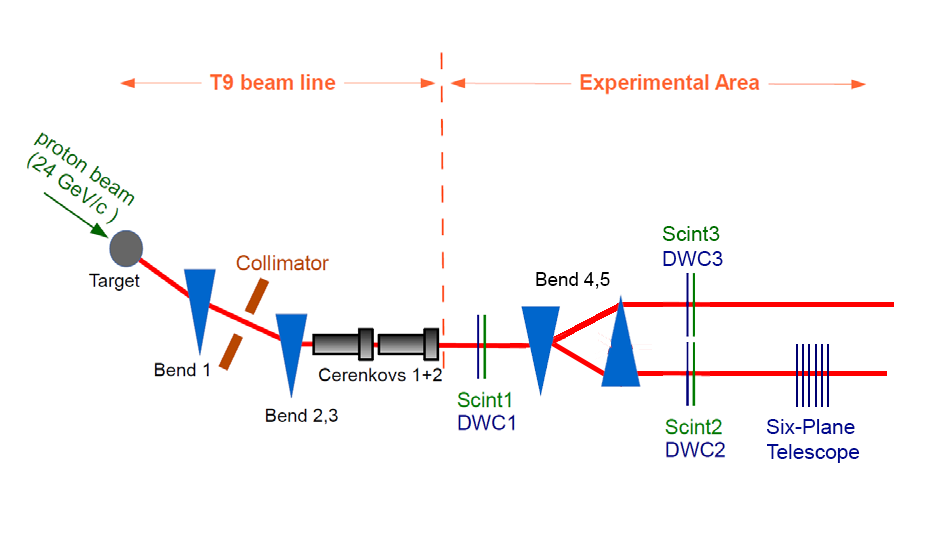
\includegraphics[]{experimental_setup3.png}
 \caption{The proposed beam line arrangement for experiment 3.}
\end{figure}

The final experiment will use an initial beam of charged particles, and split it by running it through two B-fields of equal magnitude but opposite direction.
This will produce two particle beams with opposite currents, as the positive particles are deflected one way by the B-field and the negative are deflected another.
Since the particles are oppositely charged, they would be attracted to each other due to electrostatic charges.
However, opposing currents should make them repel each other due to the induced magnetic forces. Measuring the deflection of these beams would provide insight into the effects of B-fields at relativistic velocities.

\iffalse
Quantitatively, the force on each stream of charged particles is expected to be \[
insert equation here
\]
where
\begin{description}
\item $l$ is the length of the stream of particles
\item $\lambda$ is the linear charge density
\item $d$ is the separation of the beams, and 
\item $v$ is the relative velocities of the positive and negative charge carriers
\end{description}
Here, since the charges are moving at approximately the same velocity, magnetic forces between lines are expected to be negligible and Coulombic forces are expected to dominate.
\fi
\section{Predictions}

We can make a few predictions about the measurements we'd expect from these experiments. From a stationary reference frame, a stream of charged particles resembles a current from a wire, so a B-field according to the Biot-Savart law should be expected. Thus, we predict a B-field according to
\[
	d\vec{B} = \frac{\mu_0}{4\pi}\frac{id\vec{s} \times \hat{r}}{r^2}
\]
where
\begin{description}
	\item $d\vec{B}$ is the differential B-field
	\item $\mu_0$ is the permeability constant
	\item $id\vec{s}$ is the differential current-length element
	\item $\hat{r}$ is the normalized vector from the differential current-length element to the point in space
	\item $r$ is the distance from the differential current-length element to the point in space
\end{description}

Similarly, since the drift speed of charges in current-carrying wires is so low, the forces between a current on a wire and a line of charged particles would also likely resemble those predicted by the Biot-Savart law.

\iffalse
For the first two experiments, the outcomes should be predicted by \[ %this is optional
	\vec{F_B} = i\vec{L}\times \vec{B}
\]
where
\begin{description}
	\item $\vec{F_B}$ is the force on a current due to the B-field
	\item $i$ is the current of the wire
	\item $\vec{L}$ is a length vector of the wire segment
	\item $\vec{B}$ is the B-field generated by the other current.
\end{description}
\fi

The final experiment is the most interesting. Classically, since the two lines of charged particles are negatives of each other, they can be interpretted as antiparallel currents. Therefore, the magnetic force should oppose the attractive electrostatic forces with a magnitude increasing with the velocity of the charged particles.

In the laboratory's frame of reference, the net force on the charged streams of particles is expected to decrease proportional to $1/\gamma^2$, where $\gamma$ is the Lorrentz factor. It is expected that as the velocity of the stream of particles approaches the speed of light, the net force on the particles will approach zero.

%However, since both lines are both moving at very similar velocities, there may not be very many relativistic effects between them. Thus, according to the relativistic interpretation of electromagnetism, the only forces that should exist in each of the particles' reference frames are the Coulombic forces.

\section{Motivation}
%Performing our experiment at CERN would give us more than the opportunity to test our hypotheses. It would open a galaxy of new opportunities for us.

As students, we are restricted by the limits of our textbook, the breadth of the high school curriculum, and the scarcity of our resources. We are encouraged to think outside the box. But in school, we can only think, imagine, and simulate.

The Beam Line for Schools competition gives us an opportunity to test our thinking, imagination, and simulation. 
%We already know the difficulty of devising experiments, and the massive amount of research that must be committed to understanding the physics.
The opportunity to perform experiment at CERN will help us learn more about our universe, and understand what it takes to fill the gaps in our textbooks.
It will teach us how to discover, and let us push the boundaries of human knowledge.

Simply put, we are a group of students who enjoy spending afternoons conducting experiments in our basement. We are curious. We observe the unexpected.
And we would love to have the opportunity to work with CERN’s world-renowned team of scientists.

\end{document}
